\documentclass[11pt]{article}
\usepackage[utf8]{inputenc} % Para caracteres en espa�ol
\usepackage{amsmath,amsthm,amsfonts,amssymb,amscd}
\usepackage{multirow,booktabs}
\usepackage[table]{xcolor}
\usepackage{fullpage}
\usepackage{lastpage}
\usepackage{enumitem}
\usepackage{floatrow}
\usepackage{multicol}
\usepackage{fancyhdr}
\usepackage{mathrsfs}
\usepackage{wrapfig}
\usepackage[final]{pdfpages}
\usepackage{setspace}
\usepackage{esvect}
\usepackage{calc}
\usepackage{multicol}
\usepackage{cancel}
\usepackage{graphicx}
\graphicspath{ {pictures/} }
\usepackage[retainorgcmds]{IEEEtrantools}
\usepackage[margin=3cm]{geometry}
\usepackage{amsmath}
\newlength{\tabcont}
\setlength{\parindent}{0.0in}
\setlength{\parskip}{0.05in}
\usepackage{empheq}
\usepackage{framed}
%\usepackage{newtxmath}
\usepackage{euscript}
\DeclareMathAlphabet{\mathpzc}{T1}{pzc}{m}{it}
\usepackage[most]{tcolorbox}
\usepackage{xcolor}
\colorlet{shadecolor}{orange!15}
\parindent 0in
\parskip 12pt
\geometry{margin=1in, headsep=0.25in}
\theoremstyle{definition}
\newtheorem{defn}{Definition}
\newtheorem{reg}{Rule}
\newtheorem{exer}{Exercise}
\newtheorem{note}{Note}
\newcommand{\volume}{{\ooalign{\hfil$V$\hfil\cr\kern0.08em--\hfil\cr}}}
\newcommand{\parr}{\mathbin{\|}} % Parralel Symbol
\begin{document}
\setcounter{section}{0}%Section we want -1
\setcounter{page}{1} %Page we want
\setcounter{equation}{0}%Equation we want -1
\def\thepart{\arabic{part}}
\setcounter{part}{9}
\numberwithin{equation}{part}

 \pagestyle{fancy}
\fancyhf{}
\rhead{Section 9:  Electrostatic Propulsion - Gridded Ion Engines}
\rfoot{Page \thepage}
\thispagestyle{empty}

\begin{center}
{\LARGE \bf Section 9:  Electrostatic Propulsion}\\
{\large AE435}\\
Spring 2018
\end{center}
\vspace{5mm}
\section{Gridded Ion Engines}
\vspace{25mm}
\tableofcontents
\newpage
Gridded ion engines, a.k.a. ion thrusters, are characterized by the
electrostatic acceleration of ions extracted from a plasma
generator. Ion thruster geometries are best described in terms of
three basic components:
\begin{itemize}
\item Ion accelerator
\item Plasma generator
\item Electron neutralizer
\end{itemize}
\begin{itemize}
\item Ion accelerator typically uses electrically biased multi-aperture
grids to produce the ion beam.
\item Neutralizer cathode is positioned outside the thruster body to
provide electrons to neutralize the ion beam and maintain the
potential of the thruster and spacecraft relative to the space
plasma potential.
\item Plasma generator can be direct current (DC) electron
discharges, radio frequency (RF) discharges, or microwave
discharges to produce the plasma.
\end{itemize}

\begin{center}
{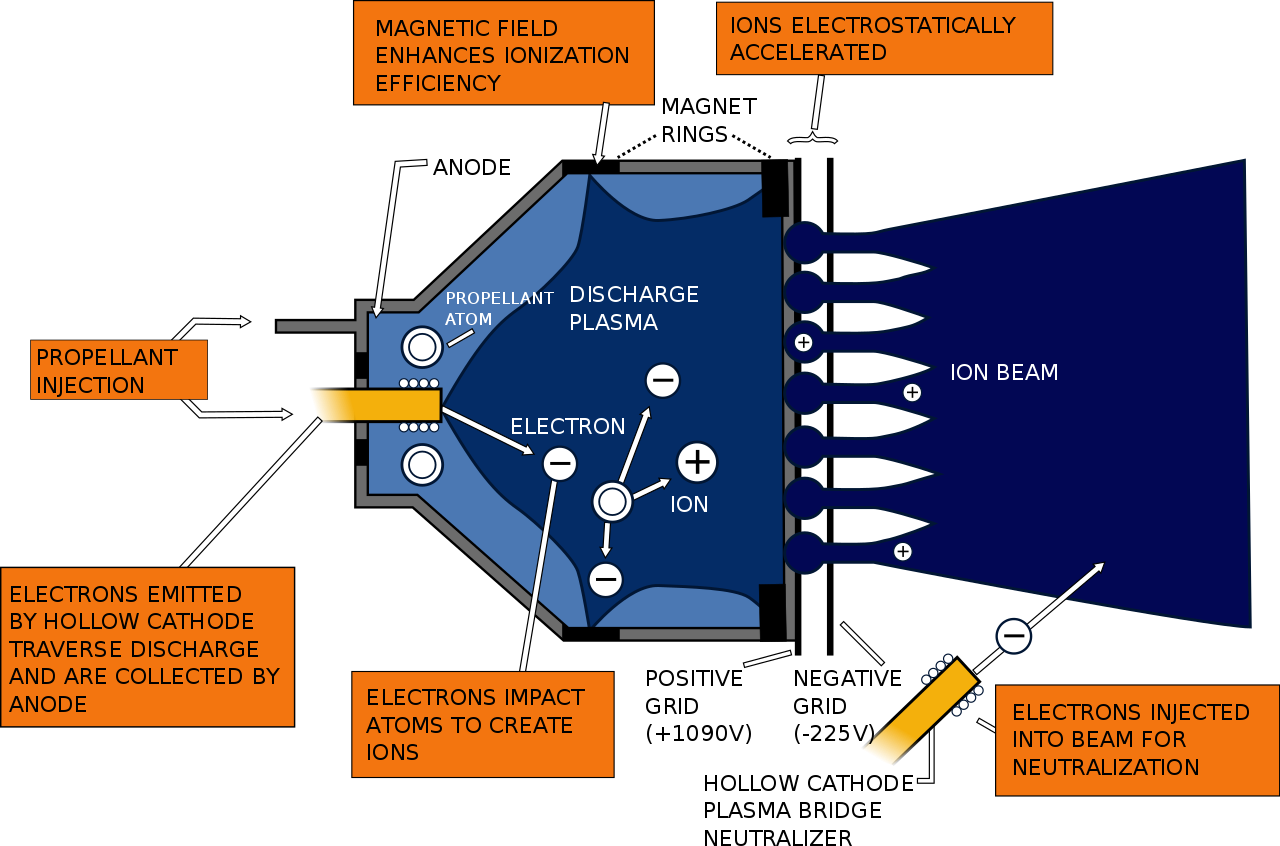
\includegraphics[scale=0.5]{1.png}}
\end{center}
\newpage
NEXIS 57-cm diameter ion engine (circa 2005), 20kW, 7000 sec,
100khr, JIMO, never flown in space

\begin{center}
{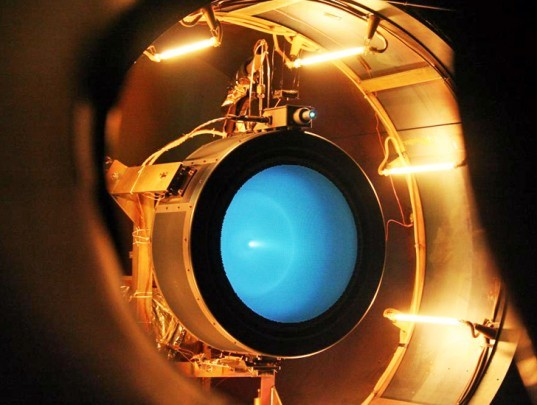
\includegraphics[scale=.7]{2.jpg}}
\end{center}

NEXT, 40-cm diameter ion engine, 7kW, 4200sec, never flown in
space


NSTAR, 30-cm diameter ion engine, 2.3kW, 3000sec, flow on
Deep-Space One in 1998 (a single unit) and DAWN in 2007 (3
units) 


\subsubsection{Electrical Schematic:}

\begin{center}
{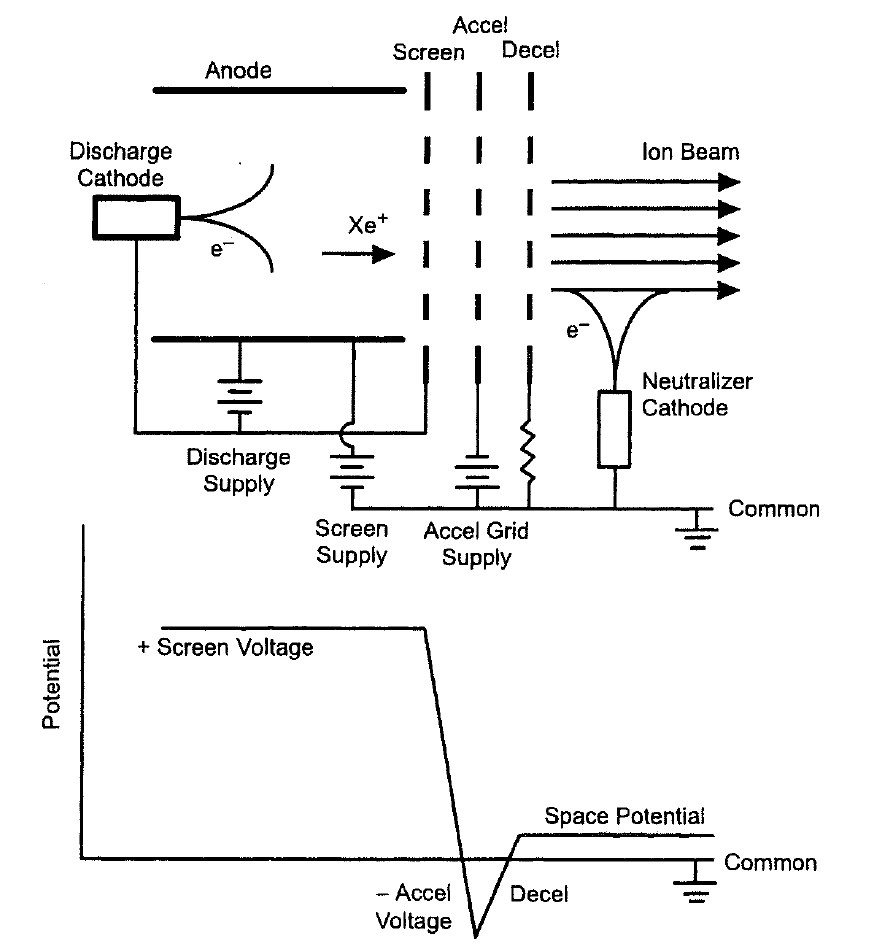
\includegraphics[scale=0.5]{3.png}}
\end{center}

Decel grid to protect accel grid from CEX ions that cause pit-ngroove
erosion of accel grid.

\newpage
\subsection{ Plasma Generator - Discharge Chamber}

The plasma generator we will focus on here is the DC electron
discharge plasma generator, typically just called the discharge
chamber. The purpose of the discharge chamber is to create a
large volume of uniform plasma from which ions can be extracted
and accelerated by the ion accelerator.

\begin{center}
{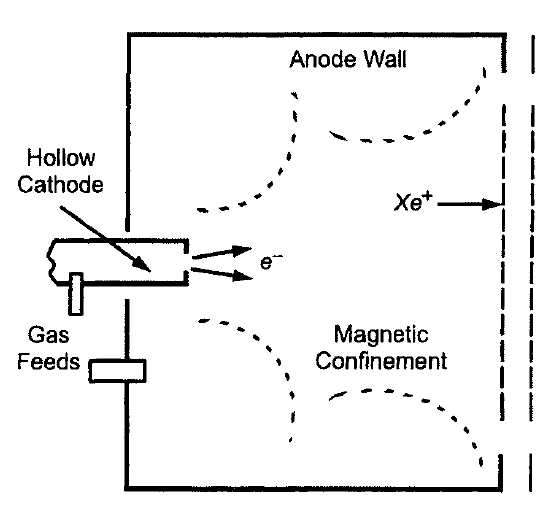
\includegraphics[scale=0.5]{4.png}}
\end{center}

\begin{center}
{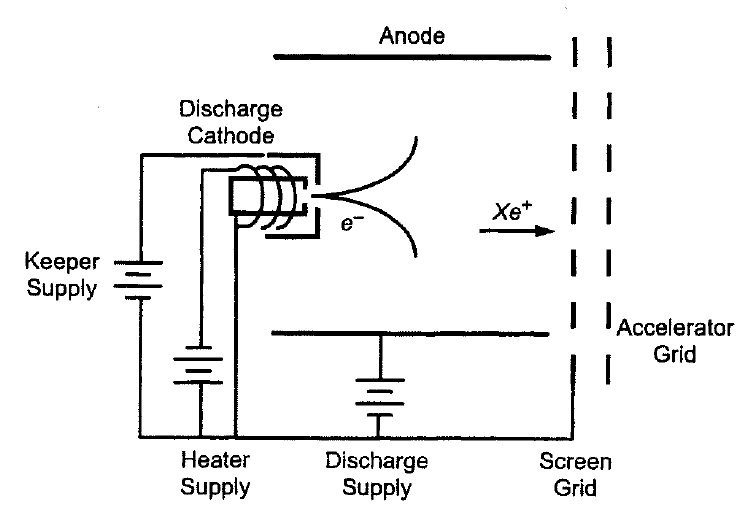
\includegraphics[scale=0.5]{5.png}}
\end{center}


The goal is to inject neutral gas atoms, ionize them, and then
supply them to the ion accelerator. Therefore there are two main
important performance metrics:

\begin{enumerate}
\item How efficiently ions are created and supplied to the accelerator.
This is called the ion production cost (or discharge loss), which
has units of eV/ion (or W/A).
\begin{equation}
\begin{aligned}
\eta_d = \frac{P_{in}}{I_b} = \frac{\text{Power In}}{\text{Beam Current}}
\end{aligned}
\end{equation}
\item How efficiently the injected neutral atoms are converted into
ions. Specifically the fraction of injected neutrals that become
supplied to the accelerator. This is called the mass utilization
efficiency.
\begin{framed}
\textbf{Mass Utilization Efficiency}
\begin{equation}
\begin{aligned}
\eta_{md} = \frac{I_b}{\frac{\dot{m}_o}{M} \, e} 
\end{aligned}
\end{equation}
Where
\begin{equation*}
\begin{aligned}
\dot{m}_o &= \text{Neutral Particle Input Flow Rate} \\
e &= \text{Electron Charge}\\
&= 1.60217662 \times10^{-19} \, C\\ 
M &= \text{Ion Mass}
\end{aligned}
\end{equation*}
\end{framed}
\end{enumerate}

Clearly we want low ion production cost (will never be less than
ionization energy! 12.13 eV/xenon-ion), and high mass utilization
efficiency.

An example of modern state-of-the-art discharge chamber is shown
here, the NEXIS ion engine.

\begin{center}
{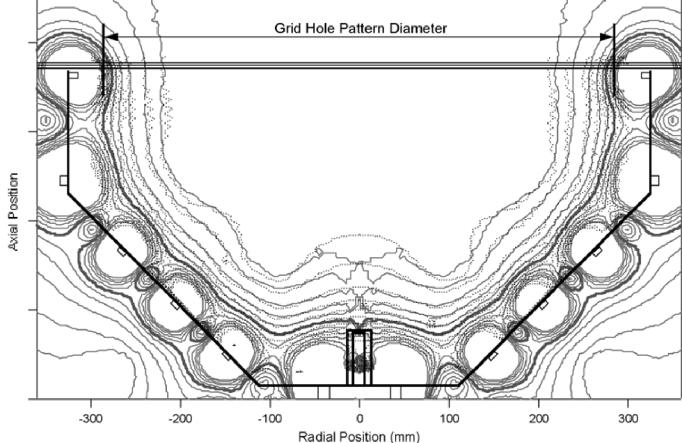
\includegraphics[scale=0.5]{6.jpg}}
\end{center}


Electrons created and emitted by the cathode (center cylinder) are
called primary electrons, and are accelerated toward the anode
body (surrounding metallic shell). These primary electrons have
ionizing collisions with neutral propellant (typically xenon, neutral
pressure of a few mTorr) injected into the chamber.

To reduce ion propulsion cost and increase mass utilization
efficiency, the pathlength of the electrons (distance they must
travel to get to the anode), and thereby their probability of having
an ionizing collision, is increased with a constant magnetic field.
A cusped field configuration has been shown to provide best
performance in terms of providing a flat beam profile with low ion
production cost and high utilization efficiency.

Cusps are created using alternating polarity of permanent (typically
samarium cobalt) magnets along the shell of the discharge
chamber. A good rule of thumb for high efficiency is to keep the
50-60 G magnetic field contour from intersecting the anode wall.

Models have been developed to predict the effect of cusp magnetic
field on electron collection at the anode, and these effects have
been incorporated into discharge chamber models. But here, we
develop a simple idealized model that neglects the magnetic field
entirely. While it is simple, it is still a good approximation to
current experimental data.

\subsubsection{Idealized Model for Predicting Discharge Chamber Performance}

Power is injected by arbitrary means into a volume filled with
neutral gas to produce ionization and neutral gas excitation.

\begin{itemize}
\item All the ions go to the grids
\item Equal number of plasma electrons go to the wall to conserve
charge.
\item Discharge chamber has a volume, V.
\end{itemize}

\begin{center}
{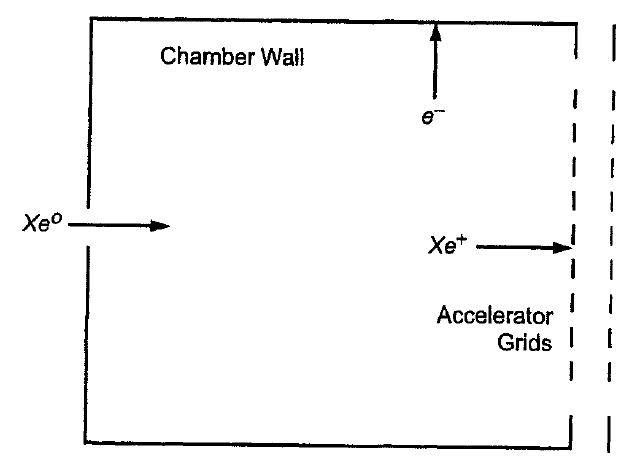
\includegraphics[scale=0.5]{7.png}}
\end{center}


Ions only flow to grids, perfect confinement everywhere else.
Current of ions to the grids is the Bohm current (due to the plasma
sheath that forms along the surface of the accelerator grids). The
Bohm current is:
\begin{shaded}
\textbf{Bohm Current}
\begin{equation}
\begin{aligned}
I_{\text{Bohm}} = I_i = \frac{1}{2} \, n_i \, e \, v_a \, A
\end{aligned}
\end{equation}
Where
\begin{equation*}
\begin{aligned}
v_a &= v_{\text{Bohm}} = \sqrt{\frac{k \, T_e}{M}} \\ 
&= \text{Ion Acoustic/Bohm Velocity} \\
A &= \text{Area of Grid}
\end{aligned}
\end{equation*}
\end{shaded}

The fraction of ions that arrive at the grids and get accelerated into
the beam is $T_g$, the "effective grid transparency", so the beam
current is:
\begin{equation}
\begin{aligned}
I_b = \frac{1}{2} \, n_i \, e \, v_a \, A \, T_g
\end{aligned}
\end{equation}
Ions in the discharge chamber are produced at a rate given by the
ionization rate coefficient:

\begin{equation}
\begin{aligned}
I_p = n_o \, n_e \, e \, <\sigma_i \, v_e> \, \volume
\end{aligned}
\end{equation}
Where
\begin{equation*}
\begin{aligned}
n_o &= \text{Neutral Density} \\
 <\sigma_i \, v_e> &= \text{Ionization Rate Coefficient; Average over Velocity Distribution Function}
\end{aligned}
\end{equation*}

Power is conserved in the system, so the power put into the plasma
is equal to the power that comes out in the form of charged
particles and radiation. To first order, the power put in goes into
ionization and excitation of neutral gas, heating of the electrons,
and power that is carried to the walls and the grids by the ions and
electrons. Then:
\begin{shaded}
\textbf{Plasma Power Input}
\begin{equation}
\begin{aligned}
P_{in} = I_p\,U^+ + I^*\,U^* + I_i \,\varepsilon_i + \frac{n_e \, \volume}{\tau} \, \varepsilon_e
\end{aligned}
\end{equation}
where

\begin{equation*}
\begin{aligned}
U^+ &= \text{Ionization potential}\\
U^* &= \text{Excitation potential}\\
\varepsilon_i &= \text{Energy carried by ions to grids}\\
\varepsilon_e &= \text{Energy carried by electrons to anode/leaving plasma}\\
I^* &= \text{Production rate of excited species}\\
\tau &= \text{Mean confinement time of electrons}\\
\end{aligned}
\end{equation*}
\end{shaded}

The production rate of excited species is given by (similar to
(9.5)):

\begin{equation}
\begin{aligned}
I^* = \sum_j \, n_o \, n_e \, e \, <\sigma^* \, v_e >_j \, \volume
\end{aligned}
\end{equation}

Where $\sigma^*$ is the cross-section for excitation to level j.

And we sum over all possible excitation levels.

Then, with (9.5), (9.7), Eqn. (9.6) becomes:

\begin{equation}
\begin{aligned}
P_{in} = n_o \, n_e \, <\sigma_i \, v_e > \, \volume \,  \bigg[U^+ + \frac{<\sigma^* \, v_e>_j}{<\sigma_i \, v_e>} \, U^* \bigg] + I_i \, \varepsilon_i + \frac{n_e \, \volume}{\tau} \, \varepsilon_e
\end{aligned}
\end{equation}

where we assume there is one "average" excited state, j, with
corresponding energy U*. (U* $\sim$ 10 eV for Xe)

Assuming the plasma is quasi-neutral ,$n_e \approx n_i$ , and that ions
and electrons leave at the same rate, such that the confinement time
of ions and electrons is the same, then:


\begin{equation}
\begin{aligned}
I_i = \frac{1}{2} \, n_i \, e \, v_a \, A = \frac{n_i \, e \, \volume}{\tau}
\end{aligned}
\end{equation}
such that:
\begin{equation}
\begin{aligned}
\tau = \frac{2 \, \volume}{v_a \, A}
\end{aligned}
\end{equation}


We see that larger volume to surface increases confinement time.
Therefore we expect discharge chambers with larger characteristic
size (e.g., radius) will have higher confinement time of charged
particles (good so electrons can have ionization collisions). Larger
discharge chambers tend to have better performance (but there's a
mass and size penalty for the spacecraft!).

Now to determine how much energy an ion and electron takes with
it when it leaves the discharge chamber, $\varepsilon_i$ and $\varepsilon_e$ . We must
consider the potential profile at the anode wall. It is an electron
repelling sheath, since the plasma potential is higher than the
anode potential.

\begin{center}
\vspace{30mm}
\textbf{Figure: Potential Profile at the Anode Wall}
\end{center}

Assuming Maxwellian electrons in the bulk plasma, these electrons
are decelerated and repelled by the sheath potential. The electron
current density reaching the wall is given by moments (integral) of
the distribution function (see 4.26):

\begin{equation}
\begin{aligned}
j_e &= e \, n \int_{-\infty}^{\infty} \, \mathrm{d}v_x \int_{-\infty}^{\infty} \, \mathrm{d}v_y \int_{\sqrt{\frac{2 \, e \, \phi}{m}}}^{\infty} \, v_z \bigg(\frac{m}{2 \, \pi \, k \, T_e}\bigg)^{\frac{3}{2}} \exp\bigg(\frac{-mv^2}{2 \, k \, T_e}\bigg)\, \mathrm{d}v_z \\ \\
&= \frac{1}{4} \, e \, n \, \sqrt{\frac{8 \, k \, T_e}{\pi \, m}} \, \exp \bigg(\frac{-e \, \phi}{k \, T_e}\bigg)
\end{aligned}
\end{equation}


The flux of kinetic energy (or kinetic power) reaching the wall is: 

\begin{equation}
\begin{aligned}
P_e &= n \int_{-\infty}^{\infty} \, \mathrm{d}v_x \int_{-\infty}^{\infty} \, \mathrm{d}v_y \int_{\sqrt{\frac{2 \, e \, \phi}{m}}}^{\infty} \, v_z \bigg(\frac{1}{2} \, m \, v^2\bigg)\bigg(\frac{m}{2 \, \pi \, k \, T_e}\bigg)^{\frac{3}{2}} \exp\bigg(\frac{-mv^2}{2 \, k \, T_e}\bigg)\, \mathrm{d}v_z
\\ \\ &= \frac{1}{4} \, n \, e \, \sqrt{\frac{8 \, k \, T_e}{\pi \, m}} \, \bigg(2 \, \frac{k \, T_e}{e} + \phi\bigg)\,\exp \bigg(\frac{-e \, \phi}{k \, T_e}\bigg)
\end{aligned}
\end{equation}


Therefore the average energy transported by an electron from the
plasma is the ratio of the power per electron to the flux of
electrons:

\begin{equation}
\begin{aligned}
\varepsilon_e = \frac{P_e}{j_e} = 2 \frac{k \, T_e}{e}+\phi = 2 \, T_{e \,[eV]} + \phi
\end{aligned}
\end{equation}


Energy removed by ions when they leave the plasma. Ions first
fall through the pre-sheath potential, which is approximately Te/2
[eV] to produce the Bohm velocity, and then through the sheath
potential, $\phi$ . Each ion then removes from the plasma a total
energy per ion of:

\begin{equation}
\begin{aligned}
\varepsilon_i =  \frac{1}{2}\, \frac{k \, T_e}{e}+\phi = \frac{1}{2} \, T_{e\,[eV]} + \phi
\end{aligned}
\end{equation}

The plasma potential, $\phi$, is found from electron current
leaving the plasma, which for a stable sheath is:

\begin{equation}
\begin{aligned}
I_{\text{anode}} = \frac{1}{4} \, \sqrt{\frac{8 \, k \, T_e}{\pi \, m}} \, e \, n_e \, A_a \, \exp\bigg(\frac{-e \, \phi}{k \, T_e}\bigg)
\end{aligned}
\end{equation}


Since we have assumed ambipolar ion and electron flow to the
wall (ion and electron loss rates are same), we can equate (9.15)
and (9.3):
\begin{shaded}
\textbf{Floating Potential}
\begin{equation}
\begin{aligned}
\phi = \frac{k \, T_e}{e} \, \ln \bigg[\frac{A_a}{A} \, \sqrt{\frac{2 \, M}{m \, \pi}}\bigg]
\end{aligned}
\end{equation}

Where

\begin{equation*}
\begin{aligned}
A &= \text{Grid Area} \\ \\
A_a &= \text{Anode Area}
\end{aligned}
\end{equation*}
\end{shaded}
This is normally called the "floating potential" since it's the
potential such that the ion and electron current are equal (we set
(9.15) equal to (9.3)). But in this model there are no applied
potentials to draw a net current.

This potential, $\phi$ , is the potential setup to balance the
electron and ion loss rate. Since electrons are less massive, they
leave the plasma first, leaving behind a slight positive charge (or
potential, $\phi$ ). This potential retards the loss of electrons to
keep the plasma quasi-neutral.

Need Electron Temperature for this model. Find electron
temperature by equating ion production and loss rates, (9.3) equal
to (9.5):

\begin{equation}
\begin{aligned}
\frac{\sqrt{\frac{k \, T_e}{M}} }{<\sigma_i \, v_e>} = \frac{2 \, n_o \, \volume}{A}
\end{aligned}
\end{equation}
Where
\begin{equation*}
\begin{aligned}
A &= \text{Ion Loss/ Grid Area} \\
n_o &= \text{Neutral Densities}
\end{aligned}
\end{equation*}

This equation can be solved for $T_e$, but not analytically. The
reaction rate coefficient has been calculated using empirically
determined collision cross-sections:

\begin{center}
{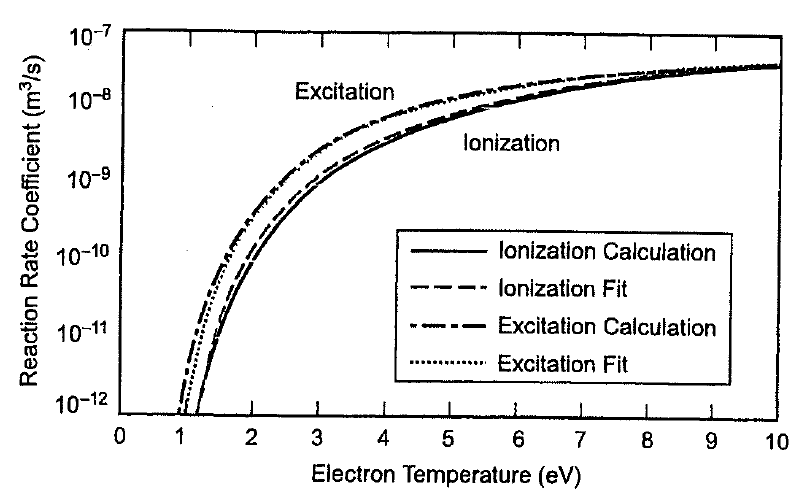
\includegraphics[scale=0.5]{8.png}}
\end{center}
\begin{center}
{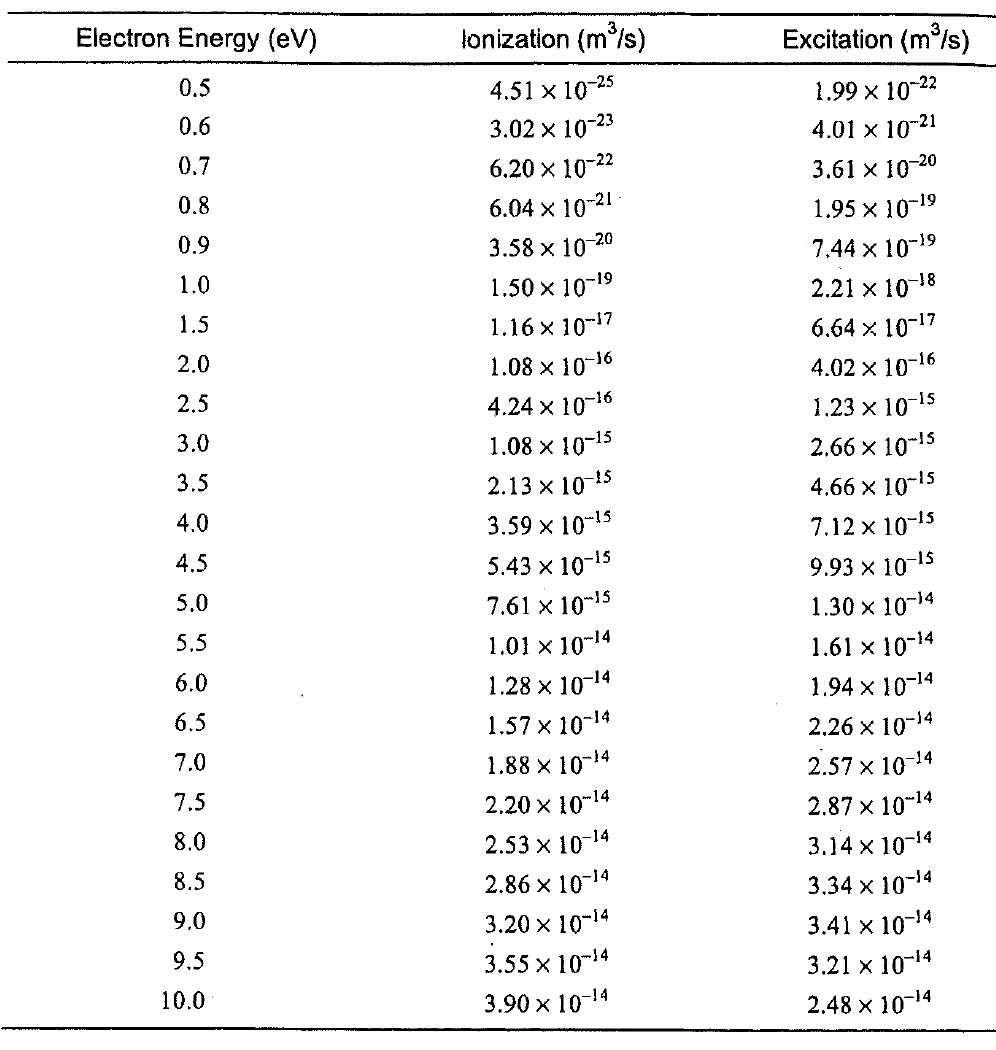
\includegraphics[scale=0.5]{9.png}}
\end{center}


Now to calculate the discharge loss (a.k.a. Ion Production Cost): 
\begin{shaded}
\textbf{Discharge Loss}
\begin{equation}
\begin{aligned}
\eta_d = \frac{P_{in}}{I_b}=\frac{2 \, n_o \, <\sigma_i \, v_e> \,\volume}{v_a \, A \, T_g} \, \bigg[U^+ + \frac{<\sigma^* \, v_e>}{<\sigma_i \, v_e>} \, U^* \bigg] + \frac{1}{T_g \, e} \Bigg[ 2.5 \, k \, T_e + 2 \, k \, T_e \, \ln \bigg(\frac{A_a}{A} \, \sqrt{\frac{2 \, M}{m \, \pi}} \bigg)\Bigg]
\end{aligned}
\end{equation}
Where
\begin{equation*}
\begin{aligned}
v_a &= v_{\text{Bohm}} = \sqrt{\frac{k \, T_e}{M}} \\ \\
M &= \text{Ion Mass}
\end{aligned}
\end{equation*}
\end{shaded}
\begin{itemize}
\item Grid transparency, $T_g$, directly affects the discharge loss
\item Input power is distributed between:
\end{itemize}

\begin{enumerate}
\item 1st term: producing ions and excited neutrals
\item 2nd term: heating the electrons that are lost to the walls
\end{enumerate}

Need the ratio of the excitation to ionization reaction rates:
\begin{center}
{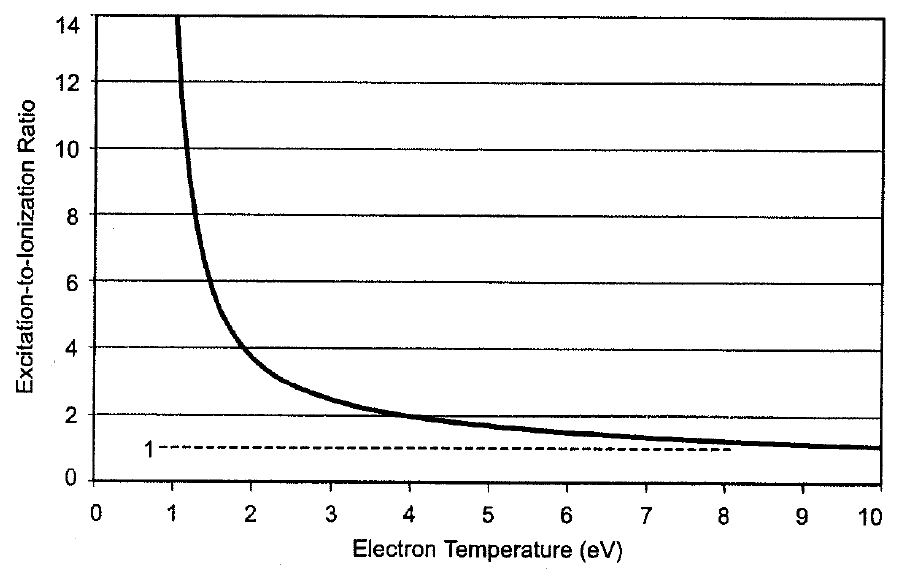
\includegraphics[scale=0.5]{10.png}}
\end{center}


At temperatures below about 8eV, the excitation rate exceeds the
ionization rate. This higher excitation rate results in more of the
power being radiated to the walls than producing ions. This
explains at least part of the inefficiency inherent in XENON
plasma generators, but similar results are found for other inert gas
propellants.

Also need Tg (~80%), xenon ionization potential (12.13 eV), xenon
excitation potential (~10 eV), diameter of grids (A), electron loss
area (Aa ~chamber wall and screen grid).

The other performance parameter is the mass utilization efficiency.
To calculate it we recognize that neutrals entering the discharge
chamber can leave the discharge chamber as neutrals through the
grid, or become ionization and leave as ions through the grids.

The mass flow rate of neutrals out of the discharge chamber can be
written as:
Neutral velocity
Neutral density
Grid area
Grid transparency to neutrals
Clausing factor

The Clausing factor accounts for the fact that the grids are finite
thickness (not infinitely thin), related to gas flow restriction in
short tubes. Typical grids have small thickness-to-length ratios, so
Clausing factor must be calculated with numerical kinetic
theory/Monte Carlo techniques, but a value of ~0.5 is typical for
ion engines.

The mass utilization efficiency was given as (9.2), which will us
(9.4) for the beam current.

Using (9.19) and (9.20), we can solve for the neutral density in the
discharge chamber:

Typical efficiencies for a discharge chamber:

20-cm diameter, 30-cm long.
\begin{center}
{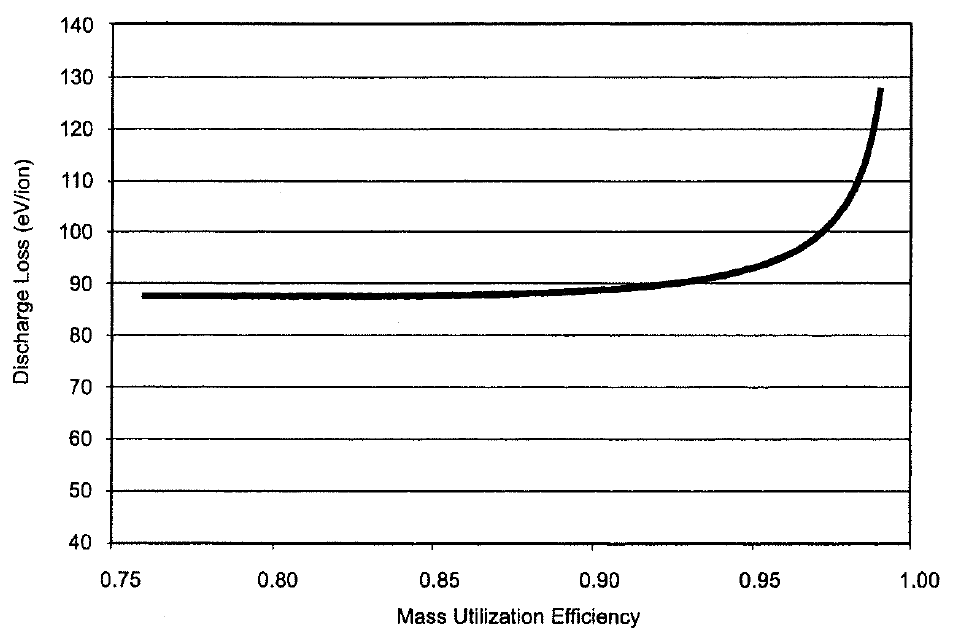
\includegraphics[scale=0.5]{11.png}}
\end{center}

Amount of power to produce 1A of beam current (with 80$\%$
transparency Tg) is about 90W. While it only takes 12.13eV to
ionize a xenon atom, even in an idealized thruster it takes 7.5 times
this energy to produce and deliver an ion into the beam due to
other losses.

What are the losses??
\begin{center}
{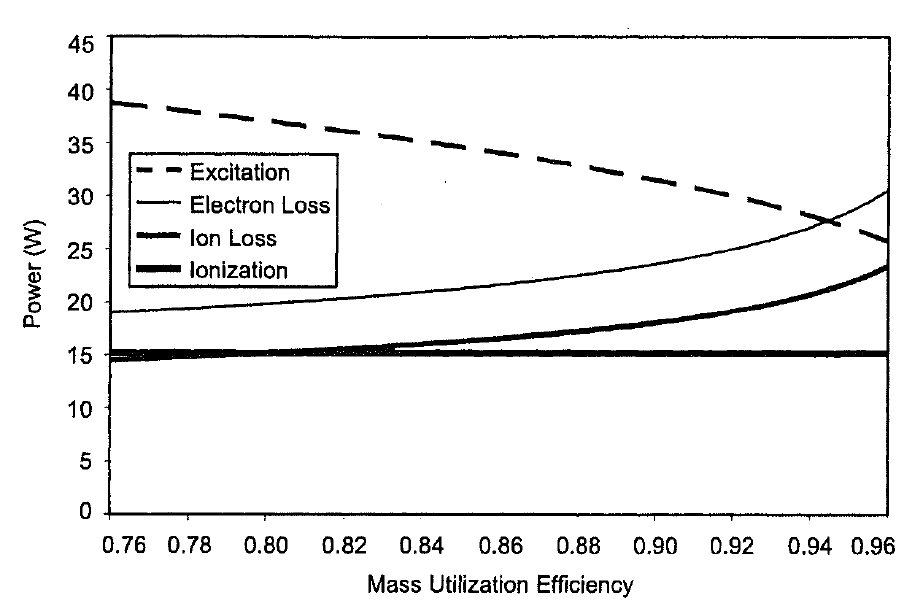
\includegraphics[scale=0.5]{12.png}}
\end{center}

This plot assumes the ionization power is constant
Major power loss is excitation at low mass utilization where
electron temp is low. Electron and ion convection losses to the
wall increase with mass utilization because there are less neutrals,
so have higher electron temp, higher plasma potential, and thereby
increased energy lost per electron and ion.

State-of-the-art discharge chambers use magnetic confinement to
reduce the effective anode area (Aa), the Bfield reduces the area of
the anode the electrons can actually get to. This effect is illustrated
below:
\begin{center}
{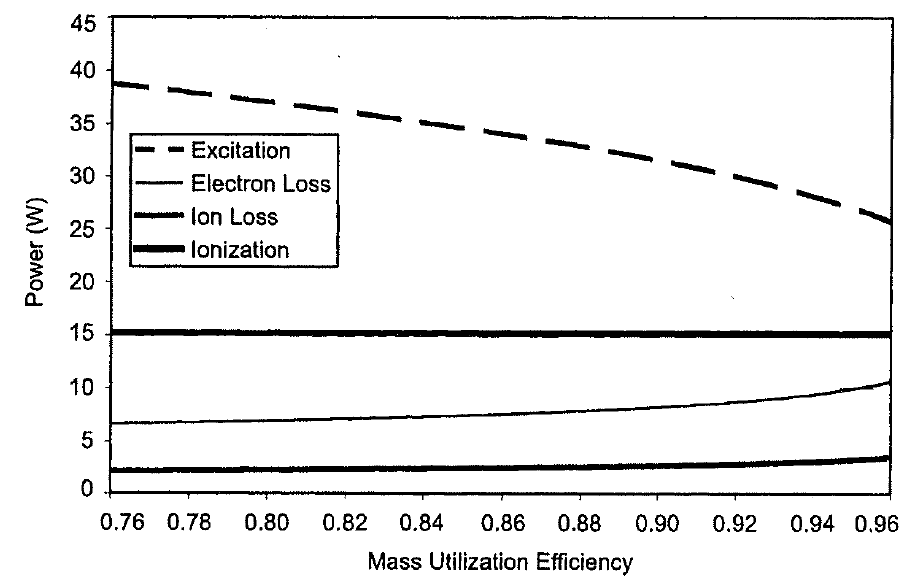
\includegraphics[scale=0.5]{13.png}}
\end{center}

Effective anode area reduced to 1$cm^2$
\end{document}